%% LaTeX .tex
%% Template para a 2ª Escola Brasileira de Dinâmica de Rotores
%% EBDR 2026
%% 17-18 de setembro de 2026, Uberlândia

\documentclass[10pt,fleqn,a4paper,twoside]{article}
\usepackage{EBDR2026}
\usepackage{array}
% babel removido para evitar option clash com o template
\usepackage[T1]{fontenc}
\usepackage[utf8]{inputenc}
%\usepackage[bottom=2cm,top=3cm,left=3cm,right=2cm]{geometry}
\usepackage{setspace}
\usepackage{indentfirst}
\usepackage{fancyhdr}
\usepackage{titlefoot}
\usepackage{tocloft}
\usepackage{titlesec}
\usepackage{enumitem}
\usepackage[bottom,stable]{footmisc}
\usepackage[hidelinks,pdfstartview=FitH]{hyperref}
\usepackage{graphicx}
\usepackage{caption}
\usepackage{subcaption}
\usepackage{multirow,multicol}
\usepackage[fleqn]{amsmath}
\usepackage{newtxtext,newtxmath}
\usepackage{physics}
\usepackage[brazilian,capitalize]{cleveref}
\usepackage{textcomp}
\usepackage{xcolor}
\usepackage{scalerel}
\usepackage{eqparbox}
\usepackage{longtable}
\usepackage{makecell}
\usepackage{threeparttable}
\usepackage{calc}
\usepackage[locale=FR]{siunitx}
\usepackage{tikz}
\usepackage{pgfplots}
\usepackage{rotating}
\usepackage{empheq}
\usepackage{pdfpages}
\usepackage{float}
\usepackage{etoolbox}
\usepackage{bibentry}

% Comando alternativo para preencher o cronograma sem depender do \cellcolor (evita conflitos com o template)
\newcommand{\gc}{\textcolor{lightgray}{\rule{6mm}{3mm}}}

\def\shortauthor{P. Autor, S. Autor e T. Autor (atualize este cabeçalho conforme necessário)}
\def\shorttitle{Título Curto do Artigo (Iniciais Maiúsculas, garantir que caiba em uma linha)}

\begin{document}
	\fphead
	
	% Cabeçalho corrigido com \parbox para evitar erros de compilação
	\noindent\hspace*{-2.5mm}\begin{tabular}{||c}
		\parbox{0.97\textwidth}{
			\vspace{2mm}
			{\centering \title{INSTRUÇÕES PARA FORMATAÇÃO DE ARTIGOS (VERSÕES PRELIMINAR E FINAL) DA EBDR 2026} \par} \vspace{4mm}
			\authors{Nome do Primeiro Autor} \\
			\authors{Nome do Segundo Autor} \\
			\institution{Instituição e endereço para o primeiro e segundo autores - se forem os mesmos} \\
			\institution{e-mails} \\
			\\
			\authors{Nome do Terceiro Autor} \\
			\institution{Instituição e endereço para o terceiro autor} \\
			\institution{e-mail} \\
			\\
			\authors{Mesmo formato para outros autores, se houver} \\
			\\
			\abstract{\textbf{Resumo.} O resumo deve descrever os objetivos, a metodologia e as principais conclusões do artigo em aproximadamente 200 palavras. Não deve conter fórmulas nem referências bibliográficas.}\\
			\\
			\keywords{\textbf{Palavras-chave:} palavra-chave 1, palavra-chave 2, palavra-chave 3\dots{} (até 5 palavras-chave)}\vspace{2mm}
		}
	\end{tabular}
	
	\section{INTRODUÇÃO}
	
	Máquinas rotativas são equipamentos amplamente utilizados no ambiente industrial. São compostas por eixos, acoplamentos, mancais, selos, discos e engrenagens. Elas têm a função de transmitir a energia mecânica para diversos equipamentos, tais como turbo-máquinas, compressores, geradores, entre outros \citep{Friswell2010}.
	
	Dessa forma, para garantir a transmissão de movimentos entre máquinas e rotores, é comum a utilização de caixas de transmissão, como exemplificado pela Fig.~\ref{fig:gearbox}. Estas são compostas por eixos contendo engrenagens, que podem ser cilíndricas ou cônicas e de dentes retos ou helicoidais.
	
	Com isso em mente, o estudo do engrenamento e como ele influencia na dinâmica de rotação torna-se importante para o completo entendimento de uma máquina rotativa ou conjunto delas \citep{stringer2008}. Assim, para a compreensão deste fenômeno, diversos modelos matemáticos foram estabelecidos, começando por modelos simples que foram se tornando mais elaborados \citep{ozguven1988}.
	
	A complexidade do modelo está associada à geometria e aos parâmetros de projeto e montagem dos pares engrenados. O intuito dos modelos de engrenamento é determinar a rigidez associada ao par engrenado, que em associação com um modelo de dinâmica de rotação, fornecerá valores de amplitude de vibração, frequências naturais, entre outros valores importantes para o cuidado da máquina e identificação de possíveis falhas \citep{kaplan2012}.
	
	\begin{figure}[H]
		\centering
		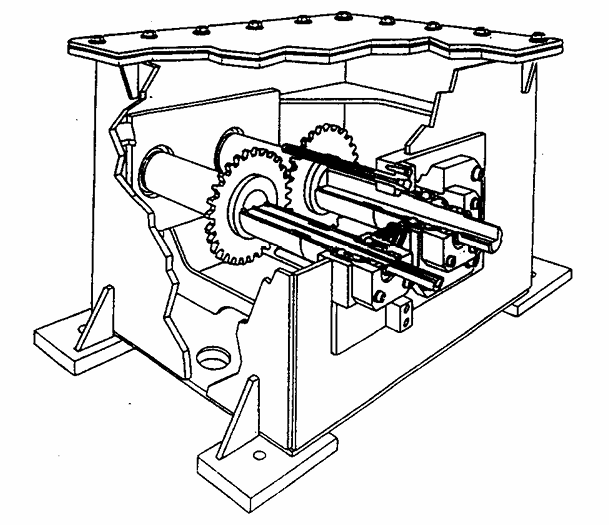
\includegraphics[width=0.5\linewidth]{imagens/gearbox.PNG}
		\caption{Exemplo de Caixa de Transmissão \cite{lim1991}.}
		\label{fig:gearbox}
	\end{figure}
	
	\subsection{Objetivo}
	Portanto, o presente trabalho visa elaborar uma metodologia de modelagem de pares engrenados que será implementada no pacote de código aberto de dinâmica de rotação \textit{Rotordynamic Open-Source Software} (ROSS) proposto por \citet{ross}.
	
	\subsubsection{Objetivos específicos}
	
	\begin{itemize}
		\item Identificar modelos de rigidez de dentes de engrenagens;
		\item Implementar metodologia para o acoplamento rotordinâmico de engrenagens;
		\item Validação da metodologia proposta com base em resultados da literatura;
		\item Adequar nova metodologia ao funcionamento do ROSS;
		\item Utilização do algoritmo implementado em casos de rotores reais.
	\end{itemize}
	
	\subsection{Justificativa}
	
	A partir da utilização de modelos de engrenamento fiéis à realidade, é possível incorporá-los à modelagem matemática e em método dos elementos finitos de rotores. Dessa maneira, com uma modelagem mais completa, fidedigna e robusta, é possível determinar amplitudes de vibração, frequências naturais, órbitas, resposta ao desbalanceamento ou outras solicitações, entre outros parâmetros. 
	
	A partir destes dados, é possível fazer um diagnóstico da operação da máquina rotativa que está sendo analisada. Dessa maneira, uma metodologia de modelagem de engrenamento torna-se um papel importante para a análise dinâmica de máquinas rotativas.
	
	\section{REVISÃO BIBLIOGRÁFICA}
	
	Neste capítulo são apresentados os conceitos fundamentais utilizados no desenvolvimento desta dissertação de mestrado. Esses conceitos incluem: a modelagem matemática da rigidez de acoplamento de um par de engrenagens e o equacionamento de rotores flexíveis, empregado na simulação e validação da implementação de engrenamento.
	
	\subsection{Modelo de rotores flexíveis}
	
	Um rotor flexível é um sistema dinâmico formado por discos, engrenagens, eixos flexíveis, mancais e selos. O modelo leva em consideração a geometria e as características de inércia, rigidez e amortecimento do sistema. Para obter a equação de movimento do rotor, os passos são: calcular a energia cinética e potencial dos componentes, escolher um método de discretização e aplicar as equações de Lagrange (Eq. \ref{eq_lalanne}) \citep{Lalanne1998}.
	
	\begin{equation}
		\frac{\mathrm{d} }{\mathrm{d} t}\left ( \frac{\partial T}{\partial \dot{q_i}} \right )-\frac{\partial T}{\partial q_i} + \frac{\partial U}{\partial q_i}=F_{qi}
		\label{eq_lalanne}
	\end{equation}
	
	Onde $N$ é o número de graus de liberdade do sistema e o índice $i$ varia entre $1 \leq i \leq N$, $q_{i}$ são as coordenadas generalizadas, $F_{qi}$ são as forças generalizadas e $T$ e $U$ são as energias cinéticas e potenciais dos componentes, respectivamente.
	
	Para este modelo, algumas considerações feitas são:
	\begin{itemize}
		\item O disco é um elemento rígido, logo possui apenas energia cinética;
		\item Engrenagens podem ser representadas como elementos de disco e estes são adicionados em nós;
		\item O eixo é representado como um elemento de viga com seção circular constante e é caracterizado por energia cinética e potencial, onde cada elemento possui dois nós e seis graus de liberdade por nó;
		\item Os mancais e selos podem ser representados por um conjunto de molas e amortecedores lineares.
	\end{itemize}
	
	Assim, a equação diferencial que representa o comportamento dinâmico de um rotor é dada pela Eq. \ref{Eq:movement}.
	
	\begin{equation}
		[M]\{\ddot{q}(t)\}+([C]+\Omega [G])\{\dot{q}(t)\}+[K]\{q(t)\}=\{F(t)\}
		\label{Eq:movement}
	\end{equation}
	
	Onde $[M]$, $[C]$, $[G]$ e $[K]$ são as matrizes de massa, amortecimento, efeito giroscópico e rigidez, respectivamente, e $\{\ddot{q}(t)\}$, $\{\dot{q}(t)\}$, $\{q(t)\}$, e $\{F(t)\}$ são os vetores de aceleração, velocidade, deslocamento e força de entrada, respectivamente. A velocidade de rotação é representada por $\Omega$.
	
	O modelo ROSS, proposto por \citet{ross}, utiliza a formulação de seis graus de liberdade para cada nó, três de translação e três de rotação, conforme mostrado abaixo.
	
	\begin{equation}
		\{q(t)\} = \{x,y,z, \theta_x, \theta_y, \theta_z\}^{T}
		\label{Eq:dof}
	\end{equation}
	
	Onde $x$, $y$ e $z$ correspondem às translações horizontal, vertical e axial, respectivamente. As variáveis $\theta_x$, $\theta_y$ e $\theta_z$ representam a flexão no plano $yz$, a flexão no plano $xz$ e a torção, respectivamente.
	
	\begin{figure}[H]
		\centering
		\begin{subfigure}[t]{0.5\textwidth}
			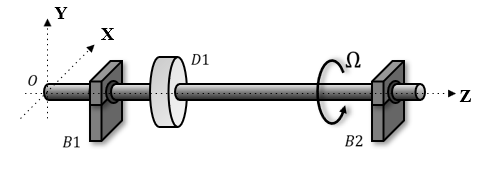
\includegraphics[width=\textwidth]{imagens/rotor1.PNG}
			\caption{Esquema de rotor}
			\label{fig:rotor1}
		\end{subfigure}
		\hfill
		\begin{subfigure}[t]{0.5\textwidth}
			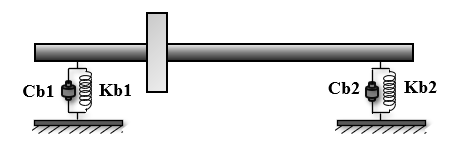
\includegraphics[width=\textwidth]{imagens/rotor2.PNG}
			\caption{Representação do modelo}
			\label{fig:rotor2}
		\end{subfigure}
		\caption{Esquema e modelo utilizado em dinâmica de rotação}
		\label{fig:rotors}
	\end{figure}
	
	\citet{jessica2025} Apresenta dados sobre a utilização mundial do pacote ROSS, juntamente com exemplos de utilização e resultados comparativos.
	
	\subsection{Rigidez do Engrenamento}
	
	Para realizar o movimento conjunto entre os rotores motor e movido, é necessário acoplar as matrizes dos dois rotores nos graus de liberdade correspondentes dos nós correspondentes, representados por $q_i$ e $q_j$. Dessa maneira, a equação do movimento pode ser modificada para Eq.~\ref{Eq:mov-alt}, já contemplando a massa, rigidez e amortecimento dos dois rotores.
	
	A Fig.~\ref{fig:mesh_repr} representa esquematicamente o engrenamento, mostrando que a rigidez de acoplamento das engrenagens $K_{mesh}$ é na direção da linha de ação e não na linha que liga os centros das duas engrenagens. A matriz de acoplamento da rigidez $[K_{mesh}]$ pode ser escrita de acordo com Eq.~\ref{Eq:k_mesh} \citep{stringer2008}.
	
	A Fig.~\ref{fig:gear_repr} apresenta a representação do par engrenado em elementos finitos. As matrizes $K_{ii}$, $K_{ij}$, $K_{ji}$ e $K_{jj}$ são apresentadas na Eq.~\ref{eq:k_matrices} de acordo com \citet{stringer2008}.
	
	\begin{figure}[H]
		\centering
		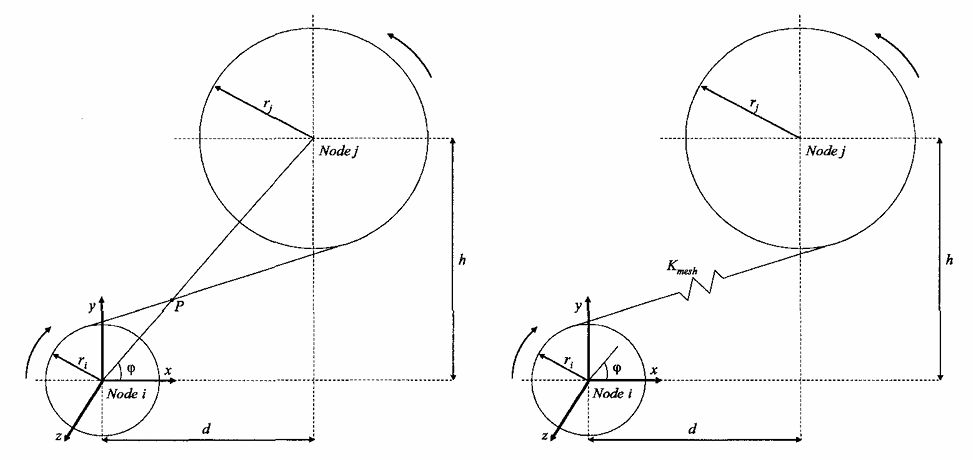
\includegraphics[width=0.8\linewidth]{imagens/gear_mesh_spring.png}
		\caption{Reapresentação do Engrenamento \citep{kaplan2012}}
		\label{fig:mesh_repr}
	\end{figure}
	
	\begin{figure}[H]
		\centering
		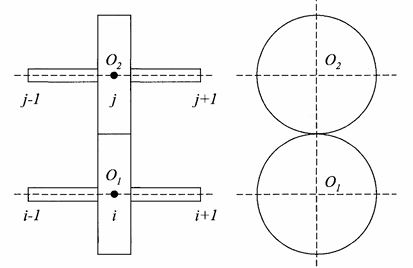
\includegraphics[width=0.6\linewidth]{imagens/gear_repr.png}
		\caption{Representação do par engrenado em elementos finitos \citep{stringer2008}}
		\label{fig:gear_repr}
	\end{figure}
	
	\begin{equation}
		[M]\{\ddot{q}(t)\}+([C]+\Omega [G])\{\dot{q}(t)\}+([K] + [K_{mesh}])\{q(t)\}=\{F(t)\}
		\label{Eq:mov-alt}
	\end{equation}
	
	\begin{equation}
		[K_{mesh}]
		\begin{Bmatrix}
			q_i \\
			q_j
		\end{Bmatrix}
		= K_{g}
		\begin{bmatrix}
			[K_{ii}] & [K_{ij}] \\
			[K_{ji}] & [K_{jj}]
		\end{bmatrix}
		\begin{Bmatrix}
			q_i \\
			q_j
		\end{Bmatrix}
		\label{Eq:k_mesh}
	\end{equation}
	
	\begin{equation}
		\label{eq:k_matrices}
		\begin{gathered}
			\resizebox{\linewidth}{!}{
				$K_{ii} = 
				\begin{bmatrix}
					(s\varphi c\phi_x + c\varphi c\phi_y)^2 & & & & & \text{sym} \\
					(s\varphi c\phi_x + c\varphi c\phi_y)(s\varphi c\phi_y - c\varphi c\phi_x) & (s\varphi c\phi_y - c\varphi c\phi_x)^2 & & & & \\
					c\phi_z(s\varphi c\phi_x + c\varphi c\phi_y) & c\phi_z(s\varphi c\phi_y - c\varphi c\phi_x) & c\phi_z^2 & & & \\
					s\varphi c\phi_z r_i(s\varphi c\phi_x + c\varphi c\phi_y) & s\varphi c\phi_z r_i(s\varphi c\phi_y - c\varphi c\phi_x) & s\varphi c\phi_z^2 r_i & (s\varphi c\phi_z r_i)^2 & & \\
					-c\varphi c\phi_z r_i(s\varphi c\phi_x + c\varphi c\phi_y) & -c\varphi c\phi_z r_i(s\varphi c\phi_y - c\varphi c\phi_x) & -c\varphi c\phi_z^2 r_i & -c\varphi s\varphi(c\phi_z r_i)^2 & (c\varphi c\phi_z r_i)^2 & \\
					-c\phi_x r_i(s\varphi c\phi_x + c\varphi c\phi_y) & -c\phi_x r_i(s\varphi c\phi_y - c\varphi c\phi_x) & -c\phi_x c\phi_z r_i & -s\varphi c\phi_x c\phi_z r_i^2 & c\varphi c\phi_x c\phi_z r_i^2 & (c\phi_x r_i)^2
				\end{bmatrix}$
			}
			\\[1.5em]
			\resizebox{\linewidth}{!}{
				$K_{ji} = 
				\begin{bmatrix}
					-(s\varphi c\phi_x + c\varphi c\phi_y)^2 & [K_{ji}]_{2,1} & [K_{ji}]_{3,1} & -s\varphi c\phi_z r_i(s\varphi c\phi_x + c\varphi c\phi_y) & c\varphi c\phi_z r_i(s\varphi c\phi_x + c\varphi c\phi_y) & c\phi_x r_i(s\varphi c\phi_x + c\varphi c\phi_y) \\
					-(s\varphi c\phi_x + c\varphi c\phi_y)(s\varphi c\phi_y - c\varphi c\phi_x) & -(s\varphi c\phi_y - c\varphi c\phi_x)^2 & [K_{ji}]_{3,2} & -s\varphi c\phi_z r_i(s\varphi c\phi_y - c\varphi c\phi_x) & c\varphi c\phi_z r_i(s\varphi c\phi_y - c\varphi c\phi_x) & c\phi_x r_i(s\varphi c\phi_y - c\varphi c\phi_x) \\
					-c\phi_z(s\varphi c\phi_x + c\varphi c\phi_y) & -c\phi_z(s\varphi c\phi_y - c\varphi c\phi_x) & -c\phi_z^2 & -s\varphi c\phi_z^2 r_i & c\varphi c\phi_z^2 r_i & c\phi_x c\phi_z r_i \\
					-s\varphi c\phi_z r_j(s\varphi c\phi_x + c\varphi c\phi_y) & -s\varphi c\phi_z r_j(s\varphi c\phi_y - c\varphi c\phi_x) & -s\varphi c\phi_z^2 r_j & -(s\varphi c\phi_z)^2 r_i r_j & c\varphi s\varphi c\phi_z^2 r_i r_j & s\varphi c\phi_x c\phi_z r_i r_j \\
					c\varphi c\phi_z r_j(s\varphi c\phi_x + c\varphi c\phi_y) & c\varphi c\phi_z r_j(s\varphi c\phi_y - c\varphi c\phi_x) & c\varphi c\phi_z^2 r_j & c\varphi s\varphi c\phi_z^2 r_i r_j & -(c\varphi c\phi_z)^2 r_i r_j & -c\varphi c\phi_x c\phi_z r_i r_j \\
					-c\phi_x r_j(s\varphi c\phi_x + c\varphi c\phi_y) & -c\phi_x r_j(s\varphi c\phi_y - c\varphi c\phi_x) & -c\phi_x c\phi_z r_j & -s\varphi c\phi_x c\phi_z r_i r_j & c\varphi c\phi_x c\phi_z r_i r_j & c\phi_x^2 r_i r_j
				\end{bmatrix}$
			}
			\\[1.5em]
			\resizebox{\linewidth}{!}{
				$K_{jj} = 
				\begin{bmatrix}
					(s\varphi c\phi_x + c\varphi c\phi_y)^2 & & & & & \text{sym} \\
					(s\varphi c\phi_x + c\varphi c\phi_y)(s\varphi c\phi_y - c\varphi c\phi_x) & (s\varphi c\phi_y - c\varphi c\phi_x)^2 & & & & \\
					c\phi_z(s\varphi c\phi_x + c\varphi c\phi_y) & c\phi_z(s\varphi c\phi_y - c\varphi c\phi_x) & c\phi_z^2 & & & \\
					s\varphi c\phi_z r_j(s\varphi c\phi_x + c\varphi c\phi_y) & s\varphi c\phi_z r_j(s\varphi c\phi_y - c\varphi c\phi_x) & s\varphi c\phi_z^2 r_j & (s\varphi c\phi_z r_j)^2 & & \\
					-c\varphi c\phi_z r_j(s\varphi c\phi_x + c\varphi c\phi_y) & -c\varphi c\phi_z r_j(s\varphi c\phi_y - c\varphi c\phi_x) & -c\varphi c\phi_z^2 r_j & -c\varphi s\varphi(c\phi_z r_j)^2 & (c\varphi c\phi_z r_j)^2 & \\
					c\phi_x r_j(s\varphi c\phi_x + c\varphi c\phi_y) & c\phi_x r_j(s\varphi c\phi_y - c\varphi c\phi_x) & c\phi_x c\phi_z r_j & s\varphi c\phi_x c\phi_z r_j^2 & -c\phi_x c\phi_z r_j^2 & (c\phi_x r_j)^2
				\end{bmatrix}$
			}
		\end{gathered}
	\end{equation}
	
	\begin{align*}
		s\varphi &= \sin\varphi, & s\varphi^2 &= (\sin\varphi)^2 \\
		c\varphi &= \cos\varphi, & c\varphi^2 &= (\cos\varphi)^2
	\end{align*}
	
	\begin{align*}
		\cos\phi_x &= \cos\beta \cos\alpha_n & \cos\phi_y &= \sin\alpha_n &   \cos\phi_z &= \sin\beta \sin\alpha_n
	\end{align*}
	
	As variáveis $q$ indicam as coordenadas generalizadas, os índices $i$ e $j$ representam os índices dos nós onde as engrenagens estão posicionadas. O parâmetro $\varphi$ representa o ângulo de orientação entre as engrenagens, $\beta$ é o ângulo de hélice das engrenagens e $\alpha_n$ representa o ângulo de pressão normal do par engrenado.
	
	Os ângulos $\phi_x$, $\phi_y$ e $\phi_z$ são de acordo com a Fig.~\ref{fig:force_component}, que representa a decomposição das forças no ponto de contato das engrenagens \citep{kaplan_paper_2013}.
	
	\begin{figure}[H]
		\centering
		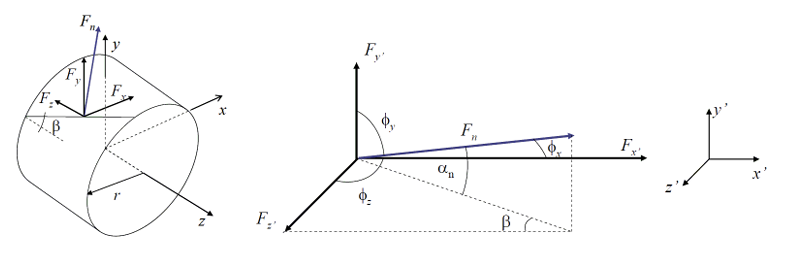
\includegraphics[width=0.9\linewidth]{imagens/force_component.png}
		\caption{Decomposição das forças no ponto de contato das engrenagens.}
		\label{fig:force_component}
	\end{figure}
	
	O parâmetro $K_g$ representa a rigidez do par engrenado ao longo da linha de ação. \citet{kaplan_paper_2013} apresenta uma metodologia de cálculo com base em parâmetros geométricos e do material das engrenagens, apresentada na Eq.~\ref{Eq:Kg}. Neste caso, é assumida a hipótese de que a rigidez dos dentes é mais significativa do que a rigidez do corpo da engrenagem.
	
	\begin{equation}
		K_g = \frac{c w E_1 E_2}{9(E_1+E_2)}
		\label{Eq:Kg}
	\end{equation}
	
	Onde $c$ representa a razão de contato do par engrenado, $w$ descreve a largura dos dentes das engrenagens, $E_1$ e $E_2$ são os módulos de elasticidade das engrenagens motriz e movida, respectivamente.
	
	\section{CRONOGRAMA DE EXECUÇÃO}

	
	\section{AGRADECIMENTOS}
	Esta seção é opcional e deve ser posicionada antes da lista de referências.
	
	\section{REFERÊNCIAS}
	
	A lista de referências deve ser apresentada como uma nova seção, localizada ao final do artigo. A primeira linha de cada referência deve ser alinhada à esquerda. Todas as demais linhas devem ter recuo de 0,5 cm a partir da margem esquerda. Todas as referências incluídas na lista devem ter sido citadas no texto. As referências devem ser listadas em ordem alfabética, de acordo com o sobrenome do primeiro autor. Veja os exemplos a seguir:
	
	\bibliographystyle{EBDR2026}
	\renewcommand{\refname}{}
	\bibliography{bibfile}
	
	\section{TERMO DE RESPONSABILIDADE}
	
	O seguinte texto, devidamente adaptado ao número de autores, deve ser incluído na última seção do artigo:
	
	O(s) autor(es) é (são) o(s) único(s) responsável(is) pelo conteúdo publicado neste artigo.
	
\end{document}